% XeLaTeX document
\documentclass[12pt,a4paper]{article}

% Редактируем: конфигурация, личные настройки: имя, название предмета и пр. для титульной страницы и метаданных документа здесь
\newcommand{\university}{Национальный исследовательский Университет ИТМО}
\newcommand{\mfaculty}{Мегафакультет информационных и трансляционных технологий}
\newcommand{\faculty}{Факультет инфокоммуникационных технологий}
\newcommand{\city}{Санкт-Петербург}
\newcommand{\num}{ №10}
\newcommand{\docname}{Лабораторная работа}
\newcommand{\subject}{Поддержка и тестирование программных модулей}
\newcommand{\tutorname}{Кононов С.С.}
\newcommand{\studentname}{Плахтий М.В.}
\newcommand{\group}{K3140}

% Не редактируем: используемые пакеты
% настройка кодировки, шрифтов и русского языка
\usepackage{fontspec}
\usepackage{polyglossia}

% рабочие ссылки в документе
\usepackage{hyperref}

% графика
\usepackage{graphicx}
\usepackage{tikz}

% поворот страницы
\usepackage{pdflscape}

% качественные листинги кода
\usepackage{minted}
\usepackage{listings}
\usepackage{lstfiracode}

% отключение копирования номеров строк из листинга, работает не во всех просмотрщиках (в Adobe Reader работает)
\usepackage{accsupp}
\newcommand\emptyaccsupp[1]{\BeginAccSupp{ActualText={}}#1\EndAccSupp{}}
\let\theHFancyVerbLine\theFancyVerbLine
\def\theFancyVerbLine{\rmfamily\tiny\emptyaccsupp{\arabic{FancyVerbLine}}}

% библиография
\bibliographystyle{templates/gost-numeric.bbx}
\usepackage{csquotes}
\usepackage[parentracker=true,backend=biber,hyperref=true,bibencoding=utf8,style=numeric-comp,language=auto,autolang=other,citestyle=gost-numeric,defernumbers=true,bibstyle=gost-numeric,sorting=ntvy]{biblatex}

% установка полей
\usepackage{geometry}

% нумерация картинок по секциям
\usepackage{chngcntr}

% дополнительные команды для таблиц
\usepackage{booktabs}

% для заголовков
\usepackage{caption}
\usepackage{titlesec}
\usepackage[dotinlabels]{titletoc}

% разное для математики
\usepackage{amsmath, amsfonts, amssymb, amsthm, mathtools}

% водяной знак на документе, см. main.tex
\usepackage[printwatermark]{xwatermark}

% Не редактируем: параметры используемых пакетов и не только
% настройки polyglossia
\setdefaultlanguage{russian}
\setotherlanguage{english}

% локализация
\addto\captionsrussian{
	\renewcommand{\figurename}{Рисунок}%
	\renewcommand{\partname}{Глава}
	\renewcommand{\contentsname}{\centerline{Содержание}}
	\renewcommand{\listingscaption}{Листинг}
}

% основной шрифт документа
\setmainfont{CMU Serif}
\newfontfamily\cyrillicfont{CMU Serif}[Script=Cyrillic]

% перечень использованных источников
\addbibresource{refs.bib}

% настройка полей
\geometry{top=2cm}
\geometry{bottom=2cm}
\geometry{left=2cm}
\geometry{right=2cm}
\geometry{bindingoffset=0cm}

% настройка ссылок и метаданных документа
\hypersetup{unicode=true,colorlinks=true,linkcolor=red,citecolor=green,filecolor=magenta,urlcolor=cyan,
	pdftitle={\docname},
	pdfauthor={\studentname},
	pdfsubject={\subject},
	pdfcreator={\studentname},
	pdfproducer={Overleaf},
	pdfkeywords={\subject}
}

% настройка подсветки кода и окружения для листингов
\usemintedstyle{colorful}
\newenvironment{code}{\captionsetup{type=listing}}{}

% шрифт для листингов с лигатурами
\setmonofont{FiraCode-Regular.otf}[
	SizeFeatures={Size=10},
	Path = templates/,
	Contextuals=Alternate
]

% оформления подписи рисунка
\captionsetup[figure]{labelsep = period}

% подпись таблицы
\DeclareCaptionFormat{hfillstart}{\hfill#1#2#3\par}
\captionsetup[table]{format=hfillstart,labelsep=newline,justification=centering,skip=-10pt,textfont=bf}

% путь к каталогу с рисунками
\graphicspath{{fig/}}

% Внесение titlepage в учёт счётчика страниц
\makeatletter
\renewenvironment{titlepage} {
	\thispagestyle{empty}
}
\makeatother

\counterwithin{figure}{section}
\counterwithin{table}{section}

\titlelabel{\thetitle.\quad}

% для удобного конспектирования математики
\mathtoolsset{showonlyrefs=true}
\theoremstyle{plain}
\newtheorem{theorem}{Теорема}[section]
\newtheorem{proposition}[theorem]{Утверждение}
\theoremstyle{definition}
\newtheorem{corollary}{Следствие}[theorem]
\newtheorem{problem}{Задача}[section]
\theoremstyle{remark}
\newtheorem*{nonum}{Решение}

% настоящее матожидание
\newcommand{\MExpect}{\mathsf{M}}

% объявили оператор!
\DeclareMathOperator{\sgn}{\mathop{sgn}}

% перенос знаков в формулах (по Львовскому)
\newcommand*{\hm}[1]{#1\nobreak\discretionary{} {\hbox{$\mathsurround=0pt #1$}}{}}


% водяной знак для обозначения статуса документа
%\newwatermark[allpages,color=red!5,angle=45,scale=3,xpos=0,ypos=0]{DRAFT}
\begin{document}
% Не редактируем: Титульная страница (формируется автоматически из заданной конфигурации)
\begin{titlepage}	% начало титульной страницы

	\begin{center}		% выравнивание по центру

		\large \university \\
		\large \mfaculty \\
		\large \faculty \\[6cm]
		% название института, затем отступ 6см

		\huge \subject \\[0.5cm] % название работы, затем отступ 0,5см
		\large \docname  \num \\[5.1cm]
		 %\large Разработка методов обучения с подкреплением\\[5cm]

	\end{center}


	\begin{flushright} % выравнивание по правому краю
		\begin{minipage}{0.25\textwidth} % врезка в половину ширины текста
			\begin{flushleft} % выровнять её содержимое по левому краю

				\large\textbf{Работу выполнил:}\\
				\large \studentname \\
				\large {Группа:} \group \\

				\large \textbf{Преподаватель:}\\
				\large \tutorname

			\end{flushleft}
		\end{minipage}
	\end{flushright}

	\vfill % заполнить всё доступное ниже пространство

	\begin{center}
		\large \city \\
		\large \the\year % вывести дату
	\end{center} % закончить выравнивание по центру

\end{titlepage} % конец титульной страницы

\vfill % заполнить всё доступное ниже пространство


% Не редактируем: Страница содержания (формируется автоматически из section, subsection и пр., указанных в content.tex)
% Содержание
\tableofcontents
\newpage



% Редактируем: всё остальное: вступление, др. этапы, заключение, приложение
\section{Описание работы программного модуля: }
\begin{itemize}
    \item На экране отображается дорога в три полосы движения.  Внизу экрана находится автомобиль.;
    \item При открытии страницы из-за верхней границы экрана вниз по одному начинают двигаться булыжники по одной из полос (имитируя движение автомобиля).;
    \item Пользователь управляет автомобилем, нажимая клавиши “A” и “D”. Автомобиль  может  находиться в трех положениях: на первой полосе, второй или третьей.; 
    \item Если автомобиль и булыжник пересекутся своими границами, вместо автомобиля и камня отобразится взрыв.;
\end{itemize}
    \begin{figure}[H]
	\begin{center}
		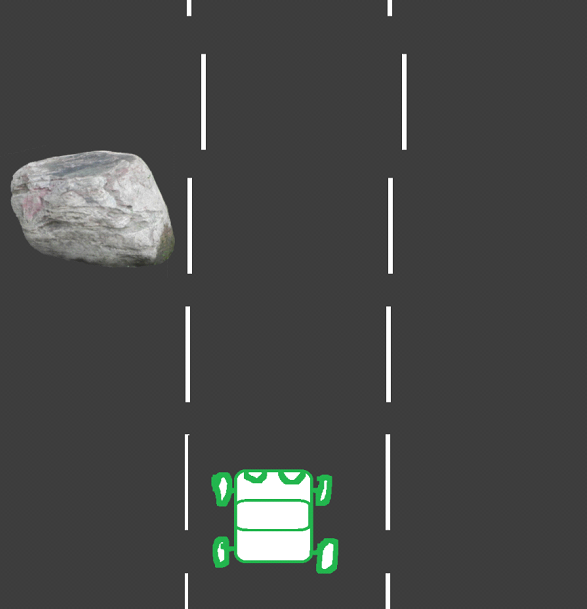
\includegraphics[scale=1]{fig/image.png}
		\caption{Внешний вид интерфейса}
		\label{pic:fig/image.png} % название для ссылок внутри кода
	\end{center}
    \end{figure}
     
    Цель Работы: провести тестирование программного модуля с использованием событий клавиатуры, написать формулу кинетической энергии до столкновения камня с машиной.

    При тестировании обращаться к \cite{ref-book}\
    
    Описание особенностей тестируемого программного модуля: В данном программном модуле особое внимание уделено использованию событий клавиатуры. 
    
    Выполненные виды тестирования: 
\begin{itemize}
    \item Тестирование функционала: ;
    \begin{itemize}
    \item Вместо камня не показывался взрыв.;
    \item После щелчка выполнялось сразу несколько условий, поэтому перемещение автомобиля работало некорректно. Был добавлен return в конце условий.;
    \item Автомобиль перемещается и после взрыва. Добавлена проверка на взрыв автомобиля.; 
\end{itemize}
\begin{code}
	\inputminted[breaklines=true, xleftmargin=1em, linenos, frame=single, framesep=10pt, fontsize=\footnotesize, firstline=1]{haskell}{listings/code.js}
	% \caption{Script.bash – bash в массы!}
    \end{code}
    \item Оценка интерфейса удобства использования веб-приложения:;

    Интерфейс приятен для восприятия

    \item Оценка кроссбраузерности:
    
Результат оценки представлен в таблице ~\ref{tab_1}
    
\end{itemize}

\begin{table}[H]
	\caption{Оценка кроссбраузерности:}
	\begin{center}
		\begin{tabular*}{\textwidth}{@{\extracolsep{\fill} } lccc}
			\toprule
			Yandex & InternetExplorer & Chrome & FireFox \\
			\midrule
			Работает корректно       & Работает корректно    & Работает корректно & Работает корректно    \\
			\bottomrule
		\end{tabular*}
		\label{tab_1}
	\end{center}
\end{table}

    \item Формула кинетической энергии  ~\ref{eq:eq1}

    
    \begin{equation}
        \centering
        \label{eq:eq1}
        K=\frac{m_{1}v_{1}^{2}}{2} + \frac{m_{2}v_{2}^{2}}{2}
    \end{equation}
    
\newpage
\section{Заключение}
Вывод: в ходе выполнения лабораторной работы было проведено тестирование программного модуля с использованием событий клавиатуры.


% Не редактируем: Страница библиографии (формируется автоматически из книжек, указанных в refs.bib и пометок \cite{имя_источника} в тексте)
\newpage
\printbibliography[title=Список использованных источников]
\addcontentsline{toc}{section}{Список использованных источников}
\end{document}
